\documentclass[conference]{IEEEtran}

\usepackage{fontspec}

\setmainfont{texgyretermes}[
    Extension = .otf,
    UprightFont = *-regular,
    ItalicFont = *-italic,
    BoldFont = *-bold,
    BoldItalicFont = *-bolditalic
]


\usepackage[english,turkish,shorthands=off]{babel}

\usepackage{cite}
\usepackage{amsmath,amssymb,amsfonts}
\usepackage{graphicx}
\usepackage{pgfplots}
\pgfplotsset{compat=1.18}
\usepgfplotslibrary{groupplots}
\usepackage{textcomp}
\usepackage{xcolor}
\usepackage{booktabs}
\usepackage[hyphens]{url}
\usepackage[hidelinks]{hyperref}

\addto\captionsturkish{%
  \renewcommand{\abstractname}{Özet}%
  \renewcommand{\IEEEkeywordsname}{Anahtar Kelimeler}%
  \renewcommand{\refname}{Kaynaklar}%
  \renewcommand{\figurename}{Şekil}%
  \renewcommand{\tablename}{TABLO}%
}
\addto\captionsenglish{%
  \renewcommand{\abstractname}{Abstract}%
  \renewcommand{\IEEEkeywordsname}{Keywords}%
}


\begin{document}

\title{C++ Ortamında Konteyner Servis Yapılandırmalarının\\
Güvenli Round-Trip Düzenlenmesi\\[3pt]
{\large\textit{Safe Round-Trip Editing of Container Service Configurations in C++}}}

\author{
\IEEEauthorblockN{Esila Şahin\textsuperscript{*,1}, Ömer Yıldız\textsuperscript{2}, Mehmet Berk Kartal\textsuperscript{3}, Ahmet Batuhan Canlı\textsuperscript{4}}
\IEEEauthorblockA{\textsuperscript{1}Yazılım Mühendisliği Bölümü, Fatih Sultan Mehmet Vakıf Üniversitesi, İstanbul, Türkiye}
\IEEEauthorblockA{\textsuperscript{2,3,4}TÜBİTAK BİLGEM UEKAE, Kocaeli, Türkiye}
\IEEEauthorblockA{\textsuperscript{*}Sorumlu yazar: esila.sahin@stu.fsm.edu.tr, ORCID: 0009-0007-8858-9540}
}

\maketitle

\begin{abstract}
Docker Compose dosyaları, geliştiricilerin yanı sıra CI/CD hatları ve
dağıtım araçları tarafından da programatik olarak değiştirilmektedir. Bu
işlem yalnızca bir YAML belgesini ayrıştırıp yeniden yazmaktan ibaret
değildir. Compose dosyaları, düzenleyici aracın modellemediği alanları,
kullanıcı tanımlı \texttt{x-*} alanlarını, kısa ve uzun sözdizimi
biçimlerini ve YAML değerlerinin tipini etkileyebilen tırnak kullanımını
içerebilir. Bu nedenle saf bir ayrıştır--değiştir--serileştir yaklaşımı,
hedeflenen değişikliğin dışında gereksiz farklar oluşturabilir veya
yapılandırma bilgisinin kaybolmasına neden olabilir. Python ve JavaScript
ekosistemlerinde biçimi korumaya yönelik YAML araçları bulunsa da, C++
tarafında Docker Compose yapılarını doğrudan ele alan ve modellenmemiş
alanların korunmasını hedefleyen ortak bir düzenleme kütüphanesi
bulunmamaktadır. Bu bildiride, Compose yapısını doğrudan temsil eden sınıf
tabanlı bir C++ API sunan ve değişiklikleri mevcut YAML düğüm ağacı üzerinde
gerçekleştiren ComposeMorph'u sunuyoruz. 647 gerçek dünya ve 38 kontrollü Compose dosyası
üzerinde yedi deneyle doğruluk, koruma, değişiklik yerelliği, ileriye
dönük uyumluluk ve performansı ölçtük. Dosyalara eklenen 802 bilinmeyen
özelliğin ve 1.203 \texttt{x-*} alanının tamamı korunmaktadır.
Değerlendirme ayrıca
yaml-cpp tabanlı serileştirmede sessiz bir tip değişimi kusuru ortaya
çıkarmıştır: tırnaklı skalerler tırnaksız yazıldığında
\texttt{docker compose config} çıktıların yalnızca \%38,1'ini kabul
etmektedir. Ayrıştırıcının sakladığı tırnak bilgisini kullanan
serileştirme bu oranı \%100'e çıkarmakta ve ölçülebilir bir performans
bedeli getirmemektedir: eşleşik ölçümde tırnak koruyan serileştirici
yaml-cpp'nin kendi serileştiricisinden \%3--21 daha hızlıdır ve en büyük
dosyalarda bile yükle--değiştir--kaydet toplamı 27 milisaniyenin altında
kalmaktadır. Kaydetmenin taban gürültüsü düşüldüğünde, ölçülen on
özelliğin tamamında düzenlemenin kendi katkısı tek satırla sınırlıdır.
Buna karşılık sağlanan koruma yapısaldır, tam anlamıyla metinsel
değildir: yorumlar ve boş satırlar korunmadığı için dosyaların yalnızca
\%4,0'ü değişiklik yapılmadan kaydedildiğinde bayt düzeyinde aynı kalır.
Ham yaml-cpp ile yapılan karşılaştırma, korumanın kaynağının bir algoritma
değil API tasarımı olduğunu göstermektedir: düzenlenen alt ağacı yeniden
inşa eden, makul görünümlü ham kod ölçülen hiçbir vakada servisin kardeş
alanlarını koruyamamıştır. Tüm veri kümeleri, betikler ve ham sonuçlar tek
komutla yeniden üretilebilir biçimde yayımlanmıştır.
\end{abstract}

\begin{IEEEkeywords}
Docker Compose; YAML round-trip düzenleme; kod olarak yapılandırma
(configuration-as-code); yapı koruma; C++
\end{IEEEkeywords}

\begin{otherlanguage}{english}
\begin{abstract}
Docker Compose files are increasingly modified programmatically by
deployment automation, continuous integration and delivery (CI/CD)
pipelines, and configuration-as-code tooling. Treating these files as
generic YAML documents is error-prone: naive parse--modify--serialize
cycles discard user-defined extension fields (\texttt{x-*}), unrecognized
properties introduced by newer Compose Specification versions, and
configuration structure unrelated to the intended change, producing
configuration churn that complicates code review. To the best of our
knowledge, no existing C++ library combines a Compose-aware, class-based
API with forward-compatible preservation of unknown and extension
properties validated through systematic round-trip testing. We present
ComposeMorph, a C++20 library that exposes typed accessors for Compose
services (image, environment, ports, volumes, networks, health checks,
deployment) while editing the underlying document tree in place, so that
untouched nodes---including unrecognized fields and \texttt{x-*}
extensions---remain structurally intact, and that writes files
atomically. We evaluate ComposeMorph in seven experiments over a
controlled corpus of 38 files and a real-world corpus of 647 Compose
files collected from GitHub, measuring round-trip correctness,
preservation, change locality, Docker Compose CLI validation success and
performance against a baseline built directly on yaml-cpp. All 802
injected unknown properties and all 1,203 \texttt{x-*} extension fields
survive a targeted single-property edit, and once the baseline save noise
is subtracted, edits stay confined to the single intended line for all
ten edited properties. The evaluation also exposes a silent type-coercion
defect in yaml-cpp-based serialization: when quoted scalars are re-emitted
unquoted, \texttt{docker compose config} accepts only 38.1\% of the
outputs. Serialization driven by the quote information the parser already
records raises this to 100\% (892/892) at no measurable performance
cost---in a paired in-process comparison the quote-preserving emitter is
3--21\% faster. Preservation is structural rather than textual: comments
and blank lines are not retained, so only 4.0\% of files are
byte-identical after an unmodified save. All datasets, scripts and raw
results are published and reproducible with a single command.
\end{abstract}

\begin{IEEEkeywords}
Docker Compose; YAML round-trip editing; configuration as code;
structure preservation; C++
\end{IEEEkeywords}
\end{otherlanguage}

\section{Giriş}
\label{sec:giris}

Docker Compose, çok konteynerli uygulamaların servislerini, ağlarını,
depolama birimlerini ve bunlar arasındaki bağımlılıkları tek bir YAML
dosyasında bildirimsel olarak tanımlamanın fiilî standardı hâline
gelmiştir~\cite{composespec}. Ibrahim ve arkadaşlarının 4.103 açık kaynak
GitHub projesi üzerinde yaptığı çalışma, Compose'un yalnızca çok bileşenli
sistemlerde değil, projelerin dörtte birinden fazlasında tek bileşenli
uygulamalar için bile kullanıldığını göstermektedir~\cite{ibrahim2021dockercompose}.
Bu dosyalar, kaynak kodla birlikte sürüm kontrolünde tutulan, elle yazılıp
bakımı yapılan birer \emph{kod olarak yapılandırma} (configuration-as-code)
varlığıdır.

Compose dosyaları artık yalnızca geliştiriciler tarafından elle
düzenlenmemekte; CI/CD hatları, kurulum araçları ve diğer dağıtım
yazılımları tarafından da programatik olarak güncellenmektedir. Örneğin
bu araçlar bir servisin \texttt{image} değerini değiştirebilir,
\texttt{environment} veya \texttt{extra\_hosts} girdileri ekleyebilir ya
da \texttt{volumes} tanımlarını hedef ortama göre güncelleyebilir. Buna
karşın C++ ekosisteminde, farklı Docker Compose yapılandırmalarını ortak ve
yeniden kullanılabilir bir API üzerinden güvenli biçimde değiştirmeye
yönelik yerleşik bir kütüphane bulunmamaktadır. Bu eksiklik çalışmanın temel
motivasyonunu oluşturmaktadır.

İlk bakışta bu tür bir düzenleme basittir: dosyayı ayrıştır, ilgili alanı
değiştir, geri yaz. Ancak bir Compose dosyası, onu düzenleyen programın
bildiği alanlardan ibaret değildir. Dosyada kullanıcı tarafından
tanımlanmış \texttt{x-*} alanları, düzenleyici aracın henüz
modellemediği daha yeni Compose Specification alanları, aynı bilginin kısa
ve uzun sözdizimi (short/long syntax) gibi farklı gösterimleri, yazarın
tırnak kullanımı ve düzen tercihleri bulunabilir. Bu nedenle saf bir
\emph{ayrıştır $\rightarrow$ değiştir $\rightarrow$ serileştir} akışı,
hedeflenen alanın çok ötesine taşan gereksiz değişikliklere
(configuration churn) ya da bilgi kaybına yol açabilir.

Üstelik bu kayıp her zaman görünür değildir. C++ tarafında akla gelen ilk
yol olan yaml-cpp~\cite{yamlcpp} tabanlı bir düzenleyici, hiçbir değişiklik
yapılmadan kaydedilen bir dosyada bile \texttt{version: "3.8"} satırının
tırnaklarını kaldırır. Ortaya çıkan \texttt{version: 3.8} ifadesi bir kayan
noktalı sayı olarak çözümlendiği için \texttt{docker compose config} dosyayı
``version must be a string'' hatasıyla reddeder. Dosya sözdizimsel olarak
geçerli bir YAML belgesidir ve düzenleyicinin kendisi tarafından sorunsuz
okunur; hata ancak Docker dosyayı okuduğunda ortaya çıkar. Kütüphanemizin
ilk sürümü de bu davranışı miras almıştı; deneylerimiz hatayı ortaya
çıkarmış, kök nedenini yaml-cpp'nin serileştiricisinde tespit etmiş ve
tırnak koruyan serileştirme (Bölüm~\ref{sec:yaklasim}) ile gidermemizi
sağlamıştır.

C++ ekosistemi bu probleme karşı özellikle hazırlıksızdır. Python'da
ruamel.yaml~\cite{ruamelyaml}, JavaScript'te eemeli/yaml~\cite{eemeliyaml}
yorumları, anahtar sırasını ve biçimi koruyan olgun round-trip desteği
sunar; Go ekosisteminde ise Compose Specification'ın başvuru kütüphanesi
compose-go~\cite{composego} ve Kubernetes araçlarının kullandığı
kyaml~\cite{kyaml} bulunur. C++ tarafında incelediğimiz YAML
kütüphanelerinin hiçbiri yorum veya biçim koruyan round-trip düzenlemeyi
desteklenen bir özellik olarak belgelememektedir: yaml-cpp'de yorumların
korunmasına yönelik talep 2015'ten beri açıktır ve kütüphanenin geliştiricisi
2026'da hâlâ böyle bir seçenek bulunmadığını belirtmiştir~\cite{yamlcpp_issue154,yamlcpp_issue457}.
İncelediğimiz C++ kütüphaneleri arasında, Docker Compose yapılarını doğrudan
modelleyen bir düzenleme API'si sunarken aynı zamanda kütüphanenin
tanımadığı Compose alanlarını korumayı sistematik olarak değerlendiren bir
çalışmaya rastlanmamıştır (Bölüm~\ref{sec:ilgili-calismalar}).

Bu bildiride, Docker Compose yapılandırmalarının C++ uygulamalarından
güvenli ve öngörülebilir biçimde değiştirilmesi için ComposeMorph adlı bir
kütüphane sunuyor ve yaklaşımın davranışını sistematik olarak
değerlendiriyoruz. ComposeMorph, yaml-cpp'nin düğüm ağacı üzerinde
\texttt{services}, \texttt{environment}, \texttt{ports},
\texttt{volumes}, \texttt{networks}, \texttt{healthcheck} ve
\texttt{deploy} gibi Compose alanlarına yönelik sınıf tabanlı bir API
sağlar. Her işlem yalnızca hedeflenen YAML düğümünü değiştirir; kütüphanenin
modellemediği alanlar yeniden oluşturulmadığı için tanınmayan Compose
alanları ve \texttt{x-*} alanları korunur. Kaydetme sırasında kaynak
dosyada tırnaklı olan skalerler yine tırnaklı yazılarak YAML tiplerinin
istemsiz biçimde değişmesi önlenir. Doğrudan modellenmeyen alanlara nokta
gösterimli yol (dot-path) üzerinden erişim sağlanır. Dosya güncellemesi ise
geçici dosyaya yazma ve atomik \texttt{rename} işlemiyle tamamlanır.

Değerlendirme; doğruluk, koruma, değişiklik yerelliği, ileriye dönük
uyumluluk ve performans başlıklı beş araştırma sorusu etrafında, 647 gerçek
dünya GitHub Compose dosyasından oluşan bir veri kümesi ile 38 kontrollü
dosyadan oluşan ikinci bir veri kümesi üzerinde yedi deneyle yapılmıştır.
Gerçek dosyalara kontrollü olarak eklenen 802 modellenmemiş Compose alanının
ve 1.203 \texttt{x-*} alanının tamamı, başka bir alan değiştirildikten sonra
da korunmuştur. \texttt{docker compose config} tarafından geçerli kabul
edilen girdilerden üretilen çıktıların tamamı (892/892) yeniden geçerli
bulunmuştur; aynı düzenlemeleri yaml-cpp'nin varsayılan serileştiricisiyle
yapan karşılaştırma sürümünde bu oran \%38,1'de (340/892) kalmaktadır. Korpustaki
9.807 tırnaklı skaler değerin hiçbiri tip değiştirmemiş, karşılaştırma sürümünde ise
452 dosyada 2.570 değer tip değiştirmiştir; 100 dosyalık bir örneklemde
çıktının girdiyle aynı veriye çözümlenme oranı 33/100'den 100/100'e
çıkmaktadır. Tırnak koruyan serileştirici
bir performans bedeli getirmez: aynı süreçte yapılan eşleşik ölçümde
yaml-cpp'nin kendi serileştiricisinden \%3--21 daha hızlıdır (Wilcoxon
işaretli sıralar testi, $p < 10^{-10}$); tek bir alanı değiştirmenin
maliyeti ise ihmal edilebilir düzeydedir. Buna karşın sağlanan koruma
yapısaldır, tam anlamıyla metinsel değildir: yorumlar ve boş satırlar
korunmadığı için dosyaların yalnızca \%4,0'ü (26/647) değişiklik yapılmadan
kaydedildiğinde bayt düzeyinde aynı kalır. Ham yaml-cpp ile yapılan
karşılaştırma, korumanın API tasarımıyla ilişkisini gösterir: aynı
düzenlemeleri ilgili alt ağacı yeniden inşa ederek yapan ham yaml-cpp kodu,
tasarımı gereği düzenlenen servisin kardeş alanlarını kaybetmiştir (0/149,
0/39, 0/116); aynı düzenlemeler ComposeMorph API'si ile hedef düğüm üzerinde yerinde
yapıldığında kardeş alanlar tüm vakalarda korunmuştur.

Bu bildirinin katkıları şunlardır:
\begin{enumerate}
  \item Docker Compose yapılandırmalarının C++ uygulamalarından sınıf
    tabanlı bir API ile düzenlenmesini sağlayan; doğrudan modellenmeyen
    alanlara genel bir erişim API'si ve atomik kaydetme desteği sunan yeniden
    kullanılabilir bir kütüphane (ComposeMorph).
  \item Hedef YAML düğümünün yerinde değiştirilmesine dayanan ve kütüphanenin
    modellemediği yeni Compose alanları ile \texttt{x-*} alanlarının
    korunmasını sağlayan yaklaşımın gerçek dünya dosyaları üzerinde
    deneysel olarak değerlendirilmesi.
  \item yaml-cpp tabanlı serileştirmede YAML değerlerinin tipini sessizce
    değiştirebilen bir problemin belirlenmesi ve giderilmesi. yaml-cpp,
    ayrıştırma sırasında tırnaklı skalerler için tuttuğu \texttt{!}
    etiketini varsayılan serileştirmede dikkate almadığından bazı string
    değerleri tırnaksız yazabilmektedir. Böyle bir değer sayı veya boolean
    olarak yeniden yorumlandığında üretilen Compose dosyası
    \texttt{docker compose config} doğrulamasından geçmeyebilmektedir.
    ComposeMorph'un tırnak bilgisini dikkate alan serileştirmesiyle doğrulama
    başarısı \%38,1'den \%100'e çıkmıştır. Aynı deneyler, kısa sözdizimiyle
    tanımlanmış \texttt{environment}, \texttt{labels} ve
    \texttt{extra\_hosts} girdilerinin düzenleme sırasında istemeden mapping
    biçimine dönüştürülmesi sorununu da ortaya çıkarmış; mevcut sözdizimini
    koruyan yerinde düzenleme ile bu davranış giderilmiştir
    (Bölüm~\ref{sec:bulgular}).
  \item 38 kontrollü ve 647 gerçek dünya Compose dosyasından oluşan iki veri
    kümesi, yedi deney ve sonuçların tek komutla yeniden üretilebilmesini
    sağlayan betiklerden oluşan tekrarlanabilir bir değerlendirme paketi.
\end{enumerate}

Bildirinin geri kalanı şöyle düzenlenmiştir. Bölüm~\ref{sec:altyapi} Docker
Compose, YAML ve round-trip düzenleme problemine ilişkin altyapıyı,
Bölüm~\ref{sec:ilgili-calismalar} ilgili çalışmaları sunar.
Bölüm~\ref{sec:tasarim} ve Bölüm~\ref{sec:yaklasim} kütüphanenin tasarımını
ve round-trip dönüşüm yaklaşımını, Bölüm~\ref{sec:gerceklestirim}
gerçekleştirimi anlatır. Bölüm~\ref{sec:yontem} deneysel yöntemi,
Bölüm~\ref{sec:bulgular} bulguları verir. Bölüm~\ref{sec:tartisma} sonuçları
tartışır; Bölüm~\ref{sec:gecerlilik} ve Bölüm~\ref{sec:kisitlamalar}
geçerlilik tehditlerini ve kısıtlamaları ele alır; Bölüm~\ref{sec:sonuc}
çalışmayı sonuçlandırır.

\section{Altyapı ve Motivasyon}
\label{sec:altyapi}

\subsection{Docker Compose Specification}
Compose Specification~\cite{composespec}, bir uygulamanın servislerini ve
bunların ağlarını, volume'larını, config ve secret tanımlarını YAML
biçiminde tanımlar. Belgenin üst seviyesinde \texttt{services},
\texttt{networks}, \texttt{volumes}, \texttt{configs}, \texttt{secrets} gibi
bölümler ile \texttt{x-} önekli \texttt{x-*} alanları bulunur. Uzantı
alanları spesifikasyonun araçlara ayırdığı resmî genişletme noktasıdır:
şema bunları serbest bırakır, ancak \texttt{x-} öneki taşımayan tanınmayan
anahtarları reddeder. Spesifikasyon ayrıca aynı bilgiyi iki biçimde ifade
etmeye izin verir. Örneğin portlar kısa sözdiziminde
\texttt{"8080:80"} biçiminde bir dizi elemanı, uzun sözdiziminde ise
\texttt{target}/\texttt{published} anahtarlarını taşıyan bir eşleme
(mapping) olarak yazılabilir; \texttt{environment}, \texttt{labels},
\texttt{extra\_hosts} ve \texttt{volumes} için de benzer ikilikler vardır.
Bir düzenleme kütüphanesi her iki biçimi de bozmadan taşımak zorundadır.

\subsection{YAML skalerleri ve örtük tip çözümlemesi}
YAML'da bir skaler değerin tipi, tırnak kullanımına bağlıdır. Tırnaksız
(plain) yazılmış \texttt{3.8} bir kayan noktalı sayı, \texttt{true} bir
boolean, \texttt{8080} bir tam sayı olarak çözümlenir; aynı değerler
tırnaklandığında string olur. YAML 1.1 çözümleme kuralları bu kümeyi
\texttt{yes}/\texttt{no}/\texttt{on}/\texttt{off} gibi boolean eşdeğerlerini,
onaltılık ve sekizlik tam sayıları, \texttt{1:30} biçimindeki altmışlık
(sexagesimal) sayıları ve tarih/zaman damgalarını da içerecek biçimde
genişletir. Dolayısıyla tırnak, YAML'da biçimsel bir tercih değil, anlam
taşıyan bir işarettir: \texttt{version: "3.8"} ile \texttt{version: 3.8}
farklı belgelerdir ve Compose şeması \texttt{version} alanının string
olmasını şart koşar.

YAML ayrıca yorum satırları, boş satırlar, girinti tercihleri, anchor/alias
(\texttt{\&ad}, \texttt{*ad}) ve birleştirme anahtarı (\texttt{<<}) gibi,
belgenin veri içeriğine değil sunumuna ait öğeler barındırır. Bu öğelerin
bir kısmı ayrıştırma sırasında veri modeline hiç taşınmaz.

\subsection{Round-trip düzenleme problemi}
Bir yapılandırma dosyasını programatik olarak düzenlemenin temel akışı
\emph{ayrıştır $\rightarrow$ değiştir $\rightarrow$ serileştir} biçimindedir.
Dosyanın bu döngü sonunda ne ölçüde korunacağı, ayrıştırıcı tarafından
tutulan ara temsile bağlıdır. Somut sözdizimi ağacı (CST) kullanan araçlar,
kaynak metindeki sözdizimsel ayrıntıları da saklayabildiği için yalnızca
değiştirilen bölümü yeniden yazabilir. ruamel.yaml~\cite{ruamelyaml} ve
eemeli/yaml~\cite{eemeliyaml} bu yaklaşım sayesinde yorum ve biçim
bilgisinin önemli bölümünü korur. yaml-cpp~\cite{yamlcpp} ise belgeyi
düzenlenebilir bir YAML düğüm ağacına dönüştürür. Bu model belge yapısını,
anahtar sırasını ve değerleri korusa da yorum, boş satır, girinti ve bazı
skaler gösterim ayrıntılarını tam olarak saklamaz. Bu nedenle dosya
kaydedilirken belgenin tamamı yeniden serileştirilir ve hedeflenen
değişikliğin dışındaki satırlarda da fark oluşabilir. Daha önemlisi,
serileştirme sırasında tırnak bilgisinin kaybedilmesi bazı skalerlerin YAML
tipinin sessizce değişmesine neden olabilir.

\subsection{İleriye dönük uyumluluk}
Compose Specification gelişmeye devam etmektedir. Bir düzenleme
kütüphanesinin nesne modeli, spesifikasyonun her sürümünü takip edemez.
Bu nedenle kütüphanenin bilmediği alanları \emph{kaybetmemesi}, yani
modellenmemiş her yapıyı olduğu gibi taşıması pratik bir gerekliliktir.
Şema temelli (dataclass/Pydantic benzeri) yaklaşımlar bu noktada
dezavantajlıdır: model, tanımadığı bir alanı saklayacak bir yere sahip
değilse serileştirmede o alan kaybolur.

\section{İlgili Çalışmalar}
\label{sec:ilgili-calismalar}

Bu bölüm, ayrıntılı taraması depoda yayımlanan sistematik inceleme
üzerine kuruludur.\footnote{\texttt{docs/related-work.md}; issue durumları
11 Eylül 2026'da GitHub API üzerinden doğrulanmıştır.}

\subsection{C ve C++ YAML kütüphaneleri}
İncelediğimiz C/C++ YAML kütüphanelerinin hiçbiri yorum veya biçim koruyan
round-trip düzenlemeyi desteklenen bir özellik olarak belgelememektedir.
yaml-cpp~\cite{yamlcpp} yorumları ayrıştırma sırasında atar; bunların
korunmasını isteyen talep 2015'ten beri açıktır~\cite{yamlcpp_issue154} ve
aynı isteği yineleyen ikinci bir kayıt 2026'da kütüphane geliştiricisi
tarafından ``şu anda böyle bir seçenek yok'' notuyla kapatılmıştır~\cite{yamlcpp_issue457}.
libyaml~\cite{libyaml} ayrıştırıcısı yorum belirteci hiç üretmez; bu,
eksik bir kolaylık API'si değil mimari bir sınırdır~\cite{libyaml_issue42}.
rapidyaml~\cite{rapidyaml} kaynağı kopyalamayan görünüm tabanlı bir tasarıma
sahiptir ve yorum koruma iddiası taşımaz; serileştiricisinde skaler tip
sadakatini bozan bir hata 2020'de bildirilmiş ve düzeltilmiştir~\cite{rapidyaml_issue30}.
O hatada serileştirici fazla tırnaklama yapmış, \texttt{-1} tam sayısını
\texttt{'-1'} string'i olarak yazmıştır; bu bildiride ölçtüğümüz tırnak
kaybının tersi yöndedir. İki durum birlikte, serileştiricinin tırnak
kararlarının C++ YAML kütüphanelerinde tekrarlayan bir tip hatası kaynağı
olduğunu göstermektedir.
fkYAML~\cite{fkyaml} başlık-tabanlı ve hızlıdır, ancak belgelerinde
round-trip koruma iddiası yoktur.

\subsection{Yorum koruyan ve CST tabanlı araçlar}
Python'da ruamel.yaml~\cite{ruamelyaml} yorumları, anahtar sırasını ve akış
biçimini \emph{yükle--değiştir--yaz} döngüsü boyunca korur.
JavaScript'te eemeli/yaml~\cite{eemeliyaml} aynı yeteneği, kaynağın her
karakterini saklayan bir CST katmanı üzerinden sunar. Rust tarafında
yaml-edit~\cite{yamledit_rust}, kayıpsız sözdizimi ağaçları için kullanılan
\texttt{rowan} altyapısına dayanarak biçim, yorum ve boşlukları korur;
benzer kayıpsız-ağaç deseni Python kaynak kodu için LibCST~\cite{libcst} ve
genel amaçlı cstree~\cite{cstree} ile de kullanılmaktadır. Bu araçların
tümü genel amaçlı YAML'a yöneliktir; hiçbiri Compose'a özgü bir nesne
modeli sunmaz ve hiçbiri C++ değildir.

\subsection{Kubernetes ve Docker Compose araçları}
Kubernetes ekosisteminde kyaml~\cite{kyaml}, manifest dosyalarını dönüştürürken
yapıyı ve yorumları korumayı hedefler; kustomize ve kpt bu kütüphane üzerine
kuruludur. Belgelenmiş sınırı, altında kullandığı go-yaml'ın yorumları her
zaman doğru işleyememesi ve bazı yorumların yanlış biçimlenmesi ya da
kaybolmasıdır~\cite{kustomize_issue259}. Docker Compose tarafında
compose-go~\cite{composego} spesifikasyonun resmî başvuru kütüphanesidir,
ancak bir yükleyici/doğrulayıcıdır; koruma odaklı bir düzenleme API'si
sunmaz. Diğer dillerde Compose dosyasını programatik olarak değiştiren
kütüphaneler mevcuttur: Go'da fishfinger~\cite{fishfinger}, Python'da
Pydantic/dataclass modelleri üzerinden çalışan compose-py~\cite{composepy},
JavaScript'te zincirlenebilir tipli bir API sunan ve bu yönüyle
ComposeMorph'un \texttt{Service} API'sine en çok benzeyen
docker-compose-yaml-parser~\cite{dockercomposeyamlparser}. Bunların hiçbiri
bilinmeyen alan veya \texttt{x-*} koruma oranını ölçülmüş bir garanti
olarak belgelemez.

\subsection{Ampirik çalışmalar}
Ibrahim ve arkadaşları 4.103 GitHub projesinde Compose kullanımını
incelemiş, dosyaların büyük bölümünün küçük ve seyrek değiştirilen
yapılandırmalar olduğunu raporlamıştır~\cite{ibrahim2021dockercompose};
Eng ve arkadaşları gerçek projelerden çok konteynerli kompozisyon
örüntülerini kataloglamıştır~\cite{eng2024patterns}. Bu çalışmalar,
GitHub kaynaklı Compose korpuslarının bu tür değerlendirmeler için
yerleşik bir veri kaynağı olduğunu göstermesi bakımından yöntemimizi
destekler. Daha geniş çerçevede, YAML'ın model yönetimi dilleriyle
işlenmesi üzerine yapılan çalışmalar~\cite{predoaia2024yaml} dönüşümü model
seviyesinde ele alır; bu bildirinin odağı ise mevcut bir dosyanın en az yan
etkiyle düzenlenmesidir.

\subsection{Konumlandırma}
İncelediğimiz çalışmalar içinde, Docker Compose yapılarını C++ tarafından
sınıf tabanlı bir API ile düzenlerken aynı zamanda araç tarafından
modellenmeyen Compose alanlarını ve \texttt{x-*} alanlarını korumayı
deneysel olarak değerlendiren bir kütüphaneye rastlanmamıştır. ComposeMorph
bu boşluğu hedeflemektedir. Bununla birlikte kütüphane, kaynak dosyanın
yorumlarını ve tüm biçimsel ayrıntılarını koruyan bir CST düzenleyicisi
değildir; bu sınırlama Bölüm~\ref{sec:kisitlamalar}'da ayrıca ele
alınmaktadır.

\section{Tasarım}
\label{sec:tasarim}

\subsection{Nesne modeli}
Kütüphanenin giriş noktası \texttt{ComposeFile} sınıfıdır: bir dosyayı
yükler, servislere ve üst seviye koleksiyonlara erişim verir, dosyayı
kaydeder. \texttt{service(ad)} çağrısı bir \texttt{Service} nesnesi
döndürür; \texttt{Service} de Compose kavramlarını doğrudan yansıtan alt
nesneler sunar (\texttt{Environment} sınıfı \texttt{labels} için de
kullanılır). Şekil~\ref{fig:model} sınıflar arasındaki ilişkiyi
göstermektedir.

\begin{figure}[t]
\centering
\begin{minipage}{0.8\columnwidth}
\footnotesize
\begin{verbatim}
ComposeFile
 +-- Service  (service(ad))
 |    +-- Environment, ExtraHosts
 |    +-- Ports, Volumes, Networks
 |    +-- BuildConfig, HealthCheck
 |    +-- DependsOn, DeployConfig
 +-- NetworkCollection, VolumeCollection
 +-- ConfigCollection, SecretCollection
\end{verbatim}
\end{minipage}
\caption{ComposeMorph nesne modeli. Her sınıf, YAML düğüm ağacındaki
ilgili düğüme tutunan ince bir görünümdür.}
\label{fig:model}
\end{figure}

Bu sınıfların hiçbiri veriyi kendi içinde kopyalamaz; her biri, altta yatan
YAML düğüm ağacının ilgili düğümüne tutunan ince bir görünümdür. Bir
\texttt{Service} nesnesi, servisin düğümüne bir tutamaçtır; üzerinde
yapılan her değişiklik doğrudan ağaçta gerçekleşir. Böylece kütüphanenin
modellemediği kardeş alanlar, düzenleme sırasında hiçbir zaman okunup
yeniden yazılmaz.

\subsection{Tipli API ile genel alan API'nin ilişkisi}
Tipli API, spesifikasyonun sık kullanılan alanlarını adlandırılmış
işlemlerle sunar; örneğin bir imaj etiketini güncellemek tek satırdır:

{\footnotesize
\begin{verbatim}
compose.service("api")
    .setImage("company/api:2.0");
\end{verbatim}
}

Modellenmemiş her alan için aynı nesne, nokta gösterimli genel bir özellik
API'si sağlar:

{\footnotesize
\begin{verbatim}
api.set("x-company-security.hsm", "enabled");
auto v = api.get<std::string>(
    "logging.options.max-file");
api.remove("deploy.placement.constraints");
\end{verbatim}
}

İki API aynı ağaç üzerinde çalışır ve birbirinin yerine geçebilir: tipli
işlemler, genel alan API'nin yapacağı düğüm yazma işleminin adlandırılmış ve
tip kontrollü bir kısayoludur. Bu ilişki, ileriye dönük uyumluluğun
kaynağıdır. Spesifikasyona yarın eklenecek bir alan için kütüphanenin
güncellenmesi gerekmez; alan genel alan API ile okunup yazılabilir, hiç
dokunulmasa bile dosyada aynen kalır.

\subsection{Kısa ve uzun sözdizimi}
Ortam değişkenleri, etiketler ve ek host kayıtları için kullanılan
sınıflar, altlarındaki düğümün liste mi yoksa eşleme mi olduğunu çalışma
zamanında tespit eder ve dosyanın mevcut biçimini korur. Örneğin ortam
değişkenleri kısa sözdiziminde, yani \texttt{KEY=value} biçimindeki liste
girdileri olarak yazılmışsa, bir değişkeni güncelleyen çağrı ilgili
girdiyi yerinde değiştirir ya da listenin sonuna yeni bir girdi ekler;
bölümü eşlemeye dönüştürmez. \texttt{Ports}, \texttt{Volumes} ve \texttt{Networks}
yardımcıları ise yalnızca kısa sözdizimli liste girdilerini destekler;
uzun sözdizimi desteği henüz yoktur (Bölüm~\ref{sec:kisitlamalar}).

\subsection{Hata yönetimi ve güvenli kaydetme}
Ayrıştırılamayan dosya, bulunamayan servis ve iş kuralı ihlali, her biri
kendi istisna türüyle bildirilir; örneğin olmayan bir servise erişim
\texttt{ServiceNotFoundException} fırlatır.
Kaydetme varsayılan olarak atomiktir: içerik önce geçici bir dosyaya
yazılır, ardından hedefin üzerine \texttt{rename} ile taşınır; böylece
yazma sırasında oluşan bir kesinti mevcut dosyayı yarım bırakmaz.
İsteğe bağlı olarak \texttt{.bak} yedeği alınabilir.

\section{Round-Trip Dönüşüm Yaklaşımı}
\label{sec:yaklasim}

\subsection{Ayrıştırma modeli ve neyin korunduğu}
ComposeMorph, belgeyi yaml-cpp'nin değiştirilebilir düğüm ağacına
ayrıştırır. Bu bir CST değildir: kaynak metnin karakter aralıkları
saklanmaz. Ağaçta korunan bilgi şunlardır: belge yapısı, eşlemelerde
anahtar sırası, koleksiyonların akış/blok stili, skaler değerlerin metni,
anchor ile paylaşılan düğümlerin kimliği ve --- bu çalışma için kritik
olan --- skalerin kaynakta tırnaksız yazılıp yazılmadığını gösteren
\emph{belirtisiz etiket}: tırnaksız (plain) skalerler \texttt{?},
tırnaklı ve blok (\texttt{|}, \texttt{>}) skalerler ise \texttt{!} etiketi
taşır. Ayrıştırmada kaybolan bilgi ise yorumlar, boş satırlar, girinti
genişliği, tek/çift tırnak ayrımı, blok skaler stili ve anchor adlarıdır.

\subsection{Değişiklik izleme ve çakışmalar}
Kütüphane bir değişiklik günlüğü tutmaz. Her düzenleme, ilgili düğüme
doğrudan yazar; dolayısıyla birleştirilecek iki sürüm ve çözülecek bir
çakışma durumu oluşmaz. Modellenmemiş alanlar hiçbir aşamada okunmaz,
kopyalanmaz veya yeniden inşa edilmez; kaydetmede ağaçta ne varsa o
yazılır. Bilinmeyen özelliklerin ve \texttt{x-*} alanlarının korunması,
ek bir mekanizmanın değil bu tasarım kararının sonucudur.

\subsection{Serileştirme}
yaml-cpp'nin varsayılan serileştiricisi bir skaleri tırnaksız yazmanın
güvenli olup olmadığına yalnızca metnine bakarak karar verir: 0.8.0
sürümünde \texttt{IsValidPlainScalar} işlevi değeri null benzeri
değerlere (\texttt{null}, \texttt{\textasciitilde}, boş string) ve
sözdizimsel olarak sakıncalı karakterlere karşı sınar, fakat boolean veya
sayı gibi görünmesini dikkate almaz. Ayrıca ayrıştırmada üretilen
\texttt{!} etiketi serileştirmede yok sayılır. Sonuç, giriş bölümünde
örneklenen davranıştır:
\texttt{version: "3.8"} tırnaksız yazılır ve yeniden okunduğunda artık
string değil kayan noktalı sayıdır.

Bu nedenle ComposeMorph, kaydetmeyi kendi ağaç yürütücüsü üzerinden yapar.
Yürütücü, yaml-cpp'nin kendi düğüm serileştiricisiyle aynı çıktıyı üretir
(aynı anchor/alias numaralandırması, aynı etiketler, aynı akış/blok stili,
aynı anahtar sırası); tek farkı skaler yazma kararıdır:

\begin{enumerate}
  \item \textbf{Birinci geçiş.} Ağaç dolaşılarak her düğümün kaç kez
    referans edildiği sayılır. Bir düğüme birden çok yoldan ulaşılıyorsa o
    düğüm anchor gerektiriyor demektir. Kimlik karşılaştırması düğüm
    kimliği üzerinden yapılır; arama uzayını daraltmak için düğümler
    kaynaktaki konumlarına göre kovalara ayrılır.
  \item \textbf{İkinci geçiş.} Ağaç yeniden dolaşılır ve yazılır. Birden
    çok referanslı bir düğüme ilk ulaşıldığında bir anchor atanır, sonraki
    ulaşımlarda alias yazılır. Eşlemeler ve diziler için düğümün stili
    (akış/blok) uygulanır.
  \item \textbf{Skaler yazma kuralı.} Düğüm \texttt{!} etiketi taşıyorsa
    (yani kaynakta tırnaklı ya da blok skaler olarak yazıldıysa) değer çift
    tırnakla yazılır; aksi
    hâlde yazma kararı yaml-cpp'nin varsayılan davranışına bırakılır.
    Böylece kaynakta tırnaksız yazılmış sayılar ve boolean'lar tırnaksız
    kalır, tırnaklı yazılmış string'ler string olarak kalır.
\end{enumerate}

\subsection{API üzerinden yazılan değerler}
Round-trip sadakati, yalnızca dosyadan gelen değerleri kapsar. API
üzerinden yazılan bir string de aynı tuzağa düşebilir: örneğin
\texttt{setCommand(\{"run", "--workers", "4"\})} çağrısında
\texttt{"4"} tırnaksız yazılırsa Compose şeması \texttt{command} dizisinin
tüm elemanlarının string olmasını beklediği için dosya reddedilir. Bu
nedenle string alan her setter, yazdığı değeri bir belirsizlik sınamasından
geçirir: değer tırnaksız yazıldığında YAML 1.1 veya YAML 1.2 çekirdek
şemasına göre null, boolean, tam sayı, kayan nokta, altmışlık sayı, zaman
damgası ya da birleştirme anahtarı olarak çözümlenecekse düğüm \texttt{!}
ile işaretlenir ve yukarıdaki kural gereği tırnaklı yazılır. Sınama
kasıtlı olarak geniş tutulmuştur: gereksiz tırnaklamanın bedeli
estetiktir, eksik tırnaklamanın bedeli sessiz tip değişimidir.

Mevcut bir değerin üzerine yazıldığında etiket korunduğu için, kaynakta
tırnaklı olan bir alan güncellendikten sonra da tırnaklı kalır; kaynakta
tırnaksız olan bir alan ise değeri belirsiz olmadıkça tırnaksız kalır.

\subsection{Desteklenmeyen YAML özellikleri}
Yorumlar ve boş satırlar ayrıştırmada kaybolduğu için çıktıda bulunmaz.
Anchor/alias yapıları korunur --- somut değerlere genişletilmez --- ancak
anchor adları ayrıştırıcı tarafından saklanmadığından çıktıda otomatik
üretilmiş sayısal adlarla (\texttt{\&1}, \texttt{*1}) yeniden yazılır.
Tek tırnaklı skalerler çift tırnakla yazılır. Blok skalerlerin
(\texttt{|}, \texttt{>}) içeriği korunur, ancak stil bilgisi
saklanmadığından değer kaçış dizileri içeren tek satırlık çift tırnaklı bir
string olarak yazılır (örneğin \texttt{"echo one\textbackslash necho two\textbackslash n"});
Veri Kümesi B'deki 647 dosyanın 55'inde (\%8,5) en az bir blok skaler
bulunmaktadır. Bu davranışlar ölçümleriyle birlikte bulgular
(Bölüm~\ref{sec:bulgular}) ve kısıtlamalar (Bölüm~\ref{sec:kisitlamalar})
bölümlerinde raporlanmaktadır.

\section{Gerçekleştirim}
\label{sec:gerceklestirim}

ComposeMorph C++20 ile yazılmıştır ve GCC 11 veya Clang 13 ve üzeri
derleyicilerle kurulabilir; değerlendirmede GCC 14.2 kullanılmıştır.
Derleme sistemi CMake (\(\geq\) 3.16), tek dış bağımlılık
yaml-cpp'dir (\(\geq\) 0.7.0; ölçümlerde 0.8.0). Birim testleri
GoogleTest ile yazılmış ve CTest'e bağlanmıştır; paket şu anda 11 test
içermektedir ve bunların dördü bu çalışmada ortaya çıkan hatalar için
yazılmış gerileme (regression) testleridir.

Kütüphanenin kendisi yaklaşık 2.100 satırdır (1.495 satır kaynak, 606
satır başlık). Değerlendirme altyapısı ayrıca beş adet C++ ölçüm aracı
(toplam 557 satır) ve on iki Python betiği (toplam yaklaşık 4.140 satır)
içerir. Depoda \texttt{src/} ve
\texttt{include/} kütüphaneyi, \texttt{benchmarks/} ölçüm araçlarını,
\texttt{datasets/} iki veri kümesini, \texttt{scripts/} deney
sürücülerini, \texttt{results/} ham çıktıları, tabloları ve figürleri,
\texttt{paper/} ise bu bildiriyi barındırır.

Docker Compose ile bütünleşme iki düzeydedir. Kütüphane içinde
\texttt{ComposeFile::validate()} temel iş kuralı denetimleri yapar
(örneğin bir servisin \texttt{image} ya da \texttt{build} alanlarından en
az birini taşıması). Asıl doğrulama ise dış araçla yapılır: üretilen her
çıktı \texttt{docker compose config} komutundan geçirilir
(Bölüm~\ref{sec:yontem}).

\section{Deneysel Yöntem}
\label{sec:yontem}

\subsection{Araştırma soruları}
\begin{itemize}
  \item \textbf{RQ1 (Doğruluk):} Kütüphane gerçek Compose dosyalarını ayrıştırıp değiştirdikten sonra geçerli Compose dosyaları üretiyor mu?
  \item \textbf{RQ2 (Koruma):} Yalnızca belirli bir alan değiştirildiğinde, değişiklikle ilgisi olmayan yapılandırma bilgisinin ne kadarı korunuyor?
  \item \textbf{RQ3 (Değişiklik yerelliği):} Hedeflenen alan değiştirilirken dosyada ne kadar gereksiz değişiklik oluşuyor?
  \item \textbf{RQ4 (İleriye dönük uyumluluk):} Nesne modelinde tanımlanmamış Compose özellikleri kaybedilmeden taşınıyor mu?
  \item \textbf{RQ5 (Performans):} Yükleme, değiştirme ve serileştirme maliyeti gerçek kullanım için kabul edilebilir mi?
\end{itemize}

\subsection{Veri kümeleri}
\textbf{Veri Kümesi A (kontrollü)}, elle yazılmış 38 dosyadan oluşur:
24 dosya Compose özelliklerini tek tek (\texttt{build}, kısa ve uzun
sözdizimli \texttt{environment}/\texttt{ports}/\texttt{volumes},
\texttt{networks}, \texttt{depends\_on}, \texttt{healthcheck},
\texttt{deploy}, \texttt{configs}, \texttt{secrets}, \texttt{labels},
\texttt{profiles}, \texttt{logging}, \texttt{sysctls}, \texttt{ulimits},
\texttt{devices}, \texttt{x-*} alanları, modellenmemiş alanlar ve iç içe
genel özellikler) izole eder; 2 dosya bunları birlikte içerir; 10 dosya
sınır durumlarını (anchor/alias ve birleştirme anahtarı, tırnaklı skaler
biçimleri, yalnızca \texttt{build} içeren servis, Unicode içerik, null ve
boş değerler, \texttt{external} kaynaklar, \texttt{extends},
\texttt{include}, yalnızca büyük/küçük harfle ayrışan anahtarlar) sınar;
2 dosya ise koruma deneylerinin işaretçi kalıplarını taşır.


\textbf{Veri Kümesi B (gerçek dünya)}, açık kaynak GitHub projelerinden
iki adımda otomatik olarak toplanmış 647 Compose dosyasından oluşur.
İlk adımda GitHub kod arama API'sinin
\texttt{filename:docker-compose.yml} sorgusundan 597, depo aramasının
\texttt{topic:docker-compose} sorgusundan 3 dosya alınmıştır; adaylar depo
ve dosya yolu düzeyinde tekilleştirilmiş, yalnızca geçerli YAML olarak
ayrıştırılan ve bir \texttt{services} eşlemesi içeren dosyalar
tutulmuştur. Bu dosyaların satır sayısı medyanı 36, en büyüğü ise 405
satırdır; büyük dosya grupları hiç temsil edilmemektedir. Bu nedenle
ikinci adımda, çok servisli yığınlar barındırma olasılığı yüksek depolarda
(homelab, self-hosted, izleme yığınları) tüm dosya ağacı taranarak 500
satırın üzerindeki 47 Compose dosyası ayrıca eklenmiştir. Dolayısıyla
korpus büyük dosyalar yönünden bilinçli olarak zenginleştirilmiştir.
Toplama ve analiz betikleri depoda yayımlanmıştır. Birleşik korpus yine de
literatürdeki gözlemlerle uyumlu biçimde küçük dosyalara eğilimlidir:
satır sayısı medyanı 39 (en büyük dosya 2.591 satır), servis sayısı
medyanı 2 (en fazla 56), üst seviye bölüm sayısı medyanı 2, YAML iç içelik
derinliği medyanı 4 ve \texttt{x-*} alanı sayısı medyanı 0'dır. Son değer, \texttt{x-*}
ve modellenmemiş alan deneylerinde neden kontrollü işaretçi enjeksiyonuna
başvurduğumuzu açıklar: bu alanlar gerçek dosyalarda doğal olarak nadirdir.

\subsection{Deneyler}
Yedi deney yürütülmüştür: (1) kimlik round-trip (değişiklik yapmadan
yükle--kaydet), (2) hedefli değişiklik ve değişiklik yerelliği (on ayrı
özellik üzerinde), (3--4) modellenmemiş alan ve \texttt{x-*} alan
koruma, (5) \texttt{docker compose config} ile doğrulama, (6) ham yaml-cpp
ile karşılaştırma, (7) performans. Her deney her iki veri kümesi üzerinde
de koşulmuştur. Deney 6'da üç araç karşılaştırılır: ComposeMorph; düğümü
yerinde değiştiren \emph{dikkatli} ham yaml-cpp kodu; ve aynı düzenlemeyi
ilgili alt ağacı yeniden inşa ederek yapan \emph{saf} ham yaml-cpp kodu.
Deney 2'de kütüphane \texttt{ports}, \texttt{extra\_hosts} ve
\texttt{networks} için yerinde değiştirme değil yalnızca ekleme ve çıkarma
işlemi sunduğundan, bu üç özellikteki hedefli değişiklik listeye tek bir
girdi eklemektir. \texttt{volume-source} düzenlemesinde en az bir kısa
sözdizimli volume girdisi bulunan servisler uygun kabul edilmiş, volume
girdilerinin tamamı uzun sözdizimli olan servisler deneyden dışlanmıştır
(Bölüm~\ref{sec:kisitlamalar}).
Dikkatli araç yaml-cpp'nin varsayılan serileştiricisini kullandığından,
Deney 5 ve tırnak analizinde aynı zamanda ``düzeltme öncesi'' sütununu
sağlar; bu eşdeğerlik ölçülmüştür (Bölüm~\ref{sec:bulgular}).

\subsection{Metrikler ve istatistiksel değerlendirme}
Metinsel koruma, girdi ile çıktı arasındaki değişen satır sayısı, değişen
satır oranı, satır düzeyinde Levenshtein uzaklığı ve normalize edilmiş
düzenleme uzaklığı ile ölçülür. Değişiklik yerelliği için
\emph{beklenen değişen satır / gerçekleşen değişen satır} oranı kullanılır;
beklenen değer tek alanlık bir düzenleme için 1'dir. Aynı dosyanın
değişiklik yapılmadan kaydedilmesindeki taban gürültü, düzeltilmiş oranda
gerçekleşen satır sayısından düşülür. Anlamsal koruma iki bağımsız
doğrulama mekanizmasıyla ölçülür: \texttt{docker compose config} (Compose şemasının
kendi doğrulayıcısı) ve PyYAML ile yeniden yükleme (değerlerin YAML
tiplerinin korunup korunmadığı). Performans ölçümleri her dosya için 30
yinelemeyle yapılır; medyan, ortalama, standart sapma ve p95 raporlanır.
İki serileştirici karşılaştırılırken ölçümler aynı süreçte, aynı ağaç
üzerinde ve yineleme başına sıra değiştirerek eşleşik biçimde alınır;
dağılım varsayımı yapmamak için Wilcoxon işaretli sıralar testi (normal
yaklaşım) kullanılır.

\subsection{Ortam ve tekrarlanabilirlik}
Ölçümler 12. nesil Intel Core i7-1255U (12 mantıksal çekirdek), 15,3 GiB
RAM, Debian GNU/Linux 13 (çekirdek 6.12), GCC 14.2.0, \texttt{Release}
derleme, C++20 ve Docker Compose 2.26.1 ortamında yapılmıştır. Tüm
deneyler depodaki tek bir komutla yeniden üretilebilir:
\texttt{./scripts/run-all-experiments.sh}. Ham çıktılar, tablolar ve
figürler \texttt{results/} altında yayımlanmıştır; düzeltme öncesi
tablolar karşılaştırma için \texttt{results/pre-fix/} altında saklanmıştır.

\section{Bulgular}
\label{sec:bulgular}

Bu bölümdeki tüm sayılar \texttt{results/tables/} altındaki üretilmiş
özetlerden alınmıştır. ``Karşılaştırma sürümü'' sütunları, aynı düzenlemeleri
yaml-cpp'nin varsayılan serileştiricisiyle yapan dikkatli ham yaml-cpp
aracına aittir; bu araç düzeltme öncesi ComposeMorph ile aynı çıktıyı
üretmektedir (100/100 dosyada bayt düzeyinde özdeş;
\texttt{results/pre-fix/tables/}).

\subsection{RQ1 --- Doğruluk}
Veri Kümesi B'deki 647 dosyanın tamamı ayrıştırılmış (647/647), kaydedilmiş
ve kaydedilen çıktı yeniden ayrıştırılabilmiştir (647/647). Veri Kümesi
A'da da 38/38 dosya için aynı sonuç alınmıştır.

Asıl ayrım dış doğrulamada ortaya çıkar. Korpustaki 647 dosyanın 491'i
(\%75,9) \texttt{docker compose config} tarafından zaten geçerli kabul
edilmektedir; kalanlar eksik \texttt{.env} dosyaları, tanımsız
interpolasyon değişkenleri veya bozuk sözdizimi gibi kütüphaneden bağımsız
nedenlerle reddedilir ve aşağıdaki oranların dışında tutulur.
Tablo~\ref{tab:validation}, bu geçerli girdilerden üretilen çıktıların
doğrulama sonuçlarını göstermektedir.

\begin{table}[t]
\caption{Docker Compose doğrulama başarı oranı (Veri Kümesi B)}
\label{tab:validation}
\centering
\begin{tabular}{lcc}
\toprule
Çıktı & ComposeMorph & Karşılaştırma sürümü \\
\midrule
Kimlik round-trip & 491/491 (\%100) & 187/491 (\%38,1) \\
Hedefli \texttt{image} düzenlemesi & 401/401 (\%100) & 153/401 (\%38,2) \\
\midrule
\textbf{Toplam} & \textbf{892/892 (\%100)} & 340/892 (\%38,1) \\
\bottomrule
\end{tabular}
\end{table}

Karşılaştırma sürümüde geçersizleşen 552 çıktının 548'i, tırnaklı bir skalerin
tırnaksız yazılması sonucu string olması gereken bir alanın sayıya veya
boolean'a dönüşmesinden kaynaklanmaktadır. Kalan 4 vakada çıktı,
Docker'ın YAML ayrıştırıcısı için sözdizimsel olarak dahi geçerli
değildir: kaynakta \texttt{":80"} biçiminde tırnaklanmış bir değer, akış
dizisi içinde tırnaksız yazıldığında PyYAML ve go-yaml tarafından
okunamamaktadır. ComposeMorph'un tırnak koruyan serileştiricisiyle bu
vakaların tamamı ortadan kalkmıştır. Veri Kümesi A'da da ComposeMorph
çıktılarının tamamı geçerlidir (64/64); karşılaştırma sürümünde yalnızca tırnaklı
skaler biçimlerini sınayan dosyanın iki çıktısı reddedilmektedir (62/64).

\subsection{RQ2 --- Koruma}
Koruma üç ayrı düzeyde ölçülmüştür.

\emph{Yapısal koruma.} Gerçek dosyalara kontrollü olarak eklenen ve
kütüphanenin modellemediği alanlar, ilgisiz bir alan değiştirildikten
sonra tüm vakalarda korunmuştur: 802/802 modellenmemiş alan ve
1.203/1.203 \texttt{x-*} alanı örneği (Veri Kümesi A'da 96/96 ve
144/144). Kontrollü sınır durumlarının altısı da (null değerli
\texttt{x-*}, skaler değerli \texttt{x-*}, liste değerli \texttt{x-*},
liste biçiminde bilinmeyen üst seviye bölüm, tipli bir bölümün içine
gömülü bilinmeyen alan, başka bir bilinmeyen bloğun içine iki düzey
gömülü \texttt{x-*}) korunmuştur.

\emph{Değer tipleri.} Korpustaki 617 dosyada açıkça tırnaklanmış 9.807
skaler değer tespit edilmiştir. ComposeMorph ile round-trip sonrasında
bunların hiçbiri tip değiştirmemiştir. Karşılaştırma sürümüde ise 452 dosyada
(tırnaklı skaler içeren dosyaların \%73,3'ü) 2.570 değer tip
değiştirmektedir: tam sayı görünümlü değerlerin \%99,9'u, kayan nokta
görünümlülerin \%100'ü ve boolean kelimelerinin \%99,5'i. Buna bağlı
olarak, çıktının girdiyle PyYAML'a göre birebir aynı veriye çözümlenme
oranı 33/100'den 100/100'e çıkmaktadır.

\emph{Metinsel koruma.} Buna karşılık çıktı bayt düzeyinde girdinin aynısı
değildir: değişiklik yapılmadan kaydedilen dosyaların yalnızca \%4,0'ü
(26/647) özdeştir; değişen satır oranının medyanı 0,167'dir (düzeltme
öncesi \%0,77 ve 0,250). Satır düzeyinde Levenshtein uzaklığının medyanı
7, normalize edilmiş düzenleme uzaklığının medyanı 0,167'dir. Kalan farklar
yorumların ve boş satırların kaybından, girinti normalizasyonundan, tek
tırnağın çift tırnağa ve blok skalerlerin tek satırlık çift tırnaklı
string'e dönüşmesinden kaynaklanır. Anchor/alias ve birleştirme anahtarı yapıları
somut değerlere genişletilmeden korunur, ancak anchor adları sayısal
adlarla yeniden yazılır.

\subsection{RQ3 --- Değişiklik Yerelliği}
On ayrı özellik üzerinde 1.467 düzenleme senaryosu koşulmuştur
(Tablo~\ref{tab:locality}). Tek alanlık bir düzenleme, ham diff'te
özelliğe göre medyan 8 ile 36 satırın değişmesine yol açmaktadır; ham
yerellik oranının medyanı bu nedenle 0,03--0,13 arasındadır. Bu satırların
neredeyse tamamı düzenlemenin kendisinden değil, kaydetmede yorum ve boş
satır kaybından ve girinti normalizasyonundan doğan taban gürültüden
kaynaklanır. Aynı dosyanın değişiklik yapılmadan kaydedilmesindeki gürültü
düşüldüğünde, on özelliğin tamamında düzeltilmiş yerellik oranının medyanı
1,0'dır: düzenlemenin kendi katkısı tek satırla sınırlıdır. Buna karşın kod
incelemesinde görülen ham diff taban gürültüyü de içerdiğinden tek
satırlık değildir (Bölüm~\ref{sec:tartisma}).

\begin{table}[t]
\caption{Özelliğe göre değişiklik yerelliği (Veri Kümesi B)}
\label{tab:locality}
\centering
\footnotesize
\setlength{\tabcolsep}{3pt}
\begin{tabular}{lrrrrr}
\toprule
 & & & Değişen & \multicolumn{2}{c}{Yerellik oranı} \\
\cmidrule(l){5-6}
Özellik & N & Başarılı & satır & Ham & Düzelt. \\
\midrule
\texttt{image} & 200 & 200 & 9 & 0,11 & 1,0 \\
\texttt{hostname} & 39 & 39 & 23 & 0,04 & 1,0 \\
\texttt{restart} & 200 & 200 & 10 & 0,10 & 1,0 \\
\texttt{env} & 200 & 200 & 9 & 0,11 & 1,0 \\
\texttt{port} & 200 & 199 & 8 & 0,13 & 1,0 \\
\texttt{volume-source} & 200 & 200 & 9 & 0,11 & 1,0 \\
\texttt{extra-host} & 34 & 34 & 36 & 0,03 & 1,0 \\
\texttt{network} & 200 & 169 & 13 & 0,08 & 1,0 \\
\texttt{healthcheck-retries} & 185 & 185 & 13 & 0,08 & 1,0 \\
\texttt{deploy-cpus} & 9 & 9 & 20 & 0,05 & 1,0 \\
\bottomrule
\end{tabular}

\smallskip
\parbox{\columnwidth}{\footnotesize Değişen satır ve oranlar medyandır.
Düzeltilmiş oran, dosyanın değişiklik yapılmadan kaydedilmesindeki
değişen satırlar düşüldükten sonra hesaplanır; 1,0 değeri düzenlemenin
yalnızca hedeflenen satırı eklediği ya da değiştirdiği anlamına gelir.}
\end{table}

Aynı ölçüm, kısa sözdizimi hatasının etkisini de ortaya koyar. Düzeltme
öncesinde, liste biçimli \texttt{environment} bölümüne sahip 94 servisin
83'ünde düzenleme, gürültü düşüldükten sonra da birden fazla satırı
değiştirmekteydi (medyan 3 satır), çünkü tek bir değişkenin güncellenmesi
listenin tamamını eşlemeye dönüştürüyordu; \texttt{extra\_hosts}'a girdi
eklemede bu sayı 9/34'tü. Düzeltmeden sonra her iki özellikte de böyle bir
vaka kalmamıştır (0/94 ve 0/34). Kısa sözdizimi hatasından etkilenmeyen
\texttt{image} düzenlemesinde bu sayı önce de sonra da sıfırdır.\footnote{Özet:
\url{results/tables/paper_supplementary_stats.md}; düzeltme öncesi ham
çıktı: \url{results/pre-fix/raw/modification_dataset_b.csv}.}

Deneyde 32 başarısızlık gözlenmiştir ve bunların tamamı kütüphanenin
bilinen bir sınırından kaynaklanır: \texttt{Networks::add} hedef düğümün
dizi olup olmadığını denetlemeden ekleme yapar, bu yüzden uzun sözdizimli
(eşleme) \texttt{networks} tanımlarında hata verir (31 vaka); benzer
biçimde \texttt{Ports::has} liste elemanlarının string olduğunu varsayar
(1 vaka). Bu sınırlar Kısıtlamalar bölümünde
(Bölüm~\ref{sec:kisitlamalar}) ayrıca ele alınmaktadır.

\subsection{RQ4 --- İleriye Dönük Uyumluluk}
Kütüphanenin nesne modelinde bulunmayan alanlar, hem \texttt{x-} önekli
\texttt{x-*} alanları hem de gelecekteki spesifikasyon alanlarını temsil eden
\texttt{x-} öneksiz modellenmemiş alanlar için tam olarak korunmuştur
(RQ2). Ancak koruma ile geçerlilik aynı şey değildir. Yalnızca
\texttt{x-*} alanları eklenen dosyaların tamamı
\texttt{docker compose config} tarafından kabul edilirken (83/83; temel
çizgide 33/83), \texttt{x-} öneksiz bilinmeyen alan eklenen dosyaların
hiçbiri kabul edilmemiştir (0/83). Bunun nedeni kütüphane değil, Compose
şemasının tanınmayan anahtarlara yalnızca \texttt{x-} öneki taşıdıklarında
izin vermesidir. Pratik sonuç şudur: ileriye dönük uyumluluk için ayrılmış
resmî mekanizma \texttt{x-*} alanlarıdır ve kütüphane bu mekanizmayı
eksiksiz desteklemektedir.

\subsection{RQ5 --- Performans}
Tablo~\ref{tab:perf}, dosya boyutuna göre yükle--değiştir--kaydet
sürelerinin medyanlarını vermektedir. Ölçümler, her boyut grubunda
alfabetik sıradaki ilk 20 dosyadan \texttt{image} düzenlemesine uygun bir
servis içerenler üzerinde yapılmıştır. Değiştirme adımının maliyeti diğer
iki adımın yanında ihmal edilebilir düzeydedir; toplam süre en büyük
dosyalarda bile onlarca milisaniye mertebesindedir. Tepe bellek kullanımı
4,7 MiB ile 8,2 MiB arasındadır.

\begin{table}[t]
\caption{Yükle--değiştir--kaydet süreleri, medyan, ms (Veri Kümesi B'den
59 dosya: 17/20/20/2; dosya başına 30 yineleme)}
\label{tab:perf}
\centering
\begin{tabular}{lrrrr}
\toprule
Grup & Yükle & Değiştir & Kaydet & Toplam \\
\midrule
Küçük ($<$100 satır) & 0,29 & 0,006 & 0,31 & 0,61 \\
Orta (100--500) & 1,31 & 0,015 & 1,12 & 2,46 \\
Büyük (500--2000) & 4,58 & 0,038 & 3,57 & 8,28 \\
Çok büyük ($>$2000) & 15,83 & 0,139 & 10,85 & 27,17 \\
\bottomrule
\end{tabular}
\end{table}

Tırnak koruyan serileştiricinin bir maliyeti olup olmadığını ölçmek için
iki serileştirici aynı süreçte, aynı ağaç üzerinde ve yineleme başına sıra
değiştirilerek karşılaştırılmıştır. ComposeMorph'un serileştiricisi tüm
boyut gruplarında yaml-cpp'nin kendi serileştiricisinden hızlıdır: medyan
oran küçük dosyalarda 0,97, orta ve büyük dosyalarda 0,94, çok büyük
dosyalarda 0,79'dur ve fark her grupta istatistiksel olarak anlamlıdır
(Wilcoxon işaretli sıralar testi, $p < 10^{-10}$). Her dosyanın ilk
yinelemesi soğuk başlangıç maliyetini içerir: sayfa hataları, dosya sistemi
önbelleği ve API üzerinden yazılan değerlerin belirsizlik sınamasında
kullanılan düzenli ifadenin süreç başına bir kez derlenmesi. İlk yinelemede
değiştirme adımının medyanı 1,26~ms'dir (59 dosyada en fazla 2,08~ms).
Bu yinelemeler istatistiklerden çıkarılmamıştır; bu nedenle ortalama ve
p95 değerleri yukarı çekilmiştir ve tipik maliyeti medyan daha iyi temsil
eder.

\subsection{Ham yaml-cpp ile karşılaştırma}
Deney 6, ComposeMorph'u iki ham yaml-cpp kullanımıyla karşılaştırır.
Serileştirme düzeyinde ComposeMorph ile dikkatli ham kullanım arasındaki
çıktı farkı 100 dosyanın 96'sında yalnızca tırnak karakterlerinden
ibarettir, 4'ünde çıktı zaten özdeştir; tırnak dışında farklılık yoktur.
Düzenleme güvenliği düzeyinde ise fark büyüktür (Şekil~\ref{fig:comparison}):
alt ağacı yeniden inşa eden saf kullanım, ölçülebilen hiçbir vakada
düzenlenen servisin diğer alanlarını koruyamamıştır (\texttt{image} için 0/149, \texttt{hostname}
için 0/39, \texttt{env} için 0/116), ComposeMorph ise tümünü korumuştur
(149/149, 39/39, 116/116). Aynı durum işaretçi alanlarında da görülür:
saf kullanım servis düzeyindeki 200 işaretçinin tamamını kaybederken üst
seviyedekilerin tamamını korur; hasar, üzerine yazılan alt ağaçla sınırlıdır.

Şekil~\ref{fig:comparison}, dikkatli ham kullanımın da kardeş alanları
her vakada korumadığını göstermektedir (130/149, 23/39, 100/116). Bu fark
yapısal bir kayıp değildir. Korunma, kardeş değerlerin düzenleme öncesi ve
sonrasında PyYAML ile karşılaştırılmasıyla ölçülür; dikkatli araç
yaml-cpp'nin varsayılan serileştiricisini kullandığından tırnaklı kardeş
değerler (ör. \texttt{"8022:22"}) tip değiştirir. Bu 51 vakanın 48'inde
kardeş alanların tümü çıktıda yerindedir ve yalnızca skaler gösterimleri
değişmiştir; kalan 3 vakada çıktı, RQ1 altında açıklanan \texttt{":80"}
sorunu nedeniyle ayrıştırılamaz hâle gelmiştir.

\begin{figure*}[t]
\centering
% Şekil kaynağın içinde çizilir; dış dosya gerekmez. Değerler:
% results/tables/comparison_summary.md, bölüm 2 (medyan değişen satır;
% korunan kardeş alan oranı = 130/149, 23/39, 100/116 vb.).
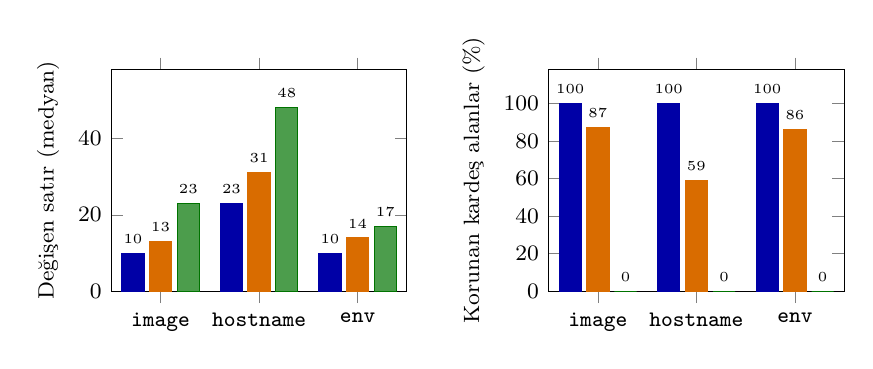
\begin{tikzpicture}
\begin{groupplot}[
  group style={group size=2 by 1, horizontal sep=1.8cm},
  width=0.44\textwidth, height=4.4cm,
  ybar, /pgf/bar width=8pt, ymin=0,
  symbolic x coords={image,hostname,env}, xtick=data,
  enlarge x limits=0.25,
  xticklabel style={font=\ttfamily\footnotesize},
  yticklabel style={font=\footnotesize},
  ylabel style={font=\footnotesize},
  nodes near coords,
  nodes near coords style={font=\tiny},
  /pgf/number format/fixed, /pgf/number format/precision=0,
  /pgf/number format/use comma,
  cycle list={
    {fill=blue!65!black, draw=blue!65!black},
    {fill=orange!85!black, draw=orange!85!black},
    {fill=green!45!black!70, draw=green!45!black}},
  area legend,
  legend style={font=\footnotesize, draw=none, fill=none,
    legend columns=3, /tikz/every even column/.append style={column sep=6pt}},
]
\nextgroupplot[ylabel={Değişen satır (medyan)}, ymax=58,
  legend to name=cmplegend]
\addplot coordinates {(image,10) (hostname,23) (env,10)};
\addplot coordinates {(image,13) (hostname,31) (env,14)};
\addplot coordinates {(image,23) (hostname,48) (env,17)};
\legend{ComposeMorph, yaml-cpp (dikkatli), yaml-cpp (naif)}
\nextgroupplot[ylabel={Korunan kardeş alanlar (\%)}, ymax=118,
  ytick={0,20,40,60,80,100}]
\addplot coordinates {(image,100) (hostname,100) (env,100)};
\addplot coordinates {(image,87.25) (hostname,58.97) (env,86.21)};
\addplot coordinates {(image,0) (hostname,0) (env,0)};
\end{groupplot}
\end{tikzpicture}

\smallskip
\ref{cmplegend}
\caption{ComposeMorph ile iki ham yaml-cpp kullanımının karşılaştırması
(Veri Kümesi B). Solda düzenleme başına değişen satır sayısının medyanı,
sağda düzenlenen servisin \emph{diğer} alanlarının korunma oranı. Alt
ağacı yeniden inşa eden saf kullanım hiçbir vakada kardeş alanları
koruyamamaktadır (\%0, çubuk görünmez). Dikkatli kullanımdaki eksik,
tırnak kaybı sonucu tip değişiminden kaynaklanır; kardeş alanlar
yapısal olarak yerindedir.}
\label{fig:comparison}
\end{figure*}

Ergonomi açısından, ComposeMorph'ta on düzenlemenin her biri tek satırdır;
aynı düzenlemeleri ham yaml-cpp ile doğru yapmak 1 ile 24 satır arasında
kod gerektirir (\texttt{volume-source} için 24, \texttt{extra-host} için
22, \texttt{env} için 18 satır). Satır sayısı hatalı kodu ayırt etmez:
\texttt{env} düzenlemesinde bölümün tamamını yeniden kuran saf sürüm
(6 satır), doğru sürümün üçte biri uzunluğundadır. \texttt{image} ve
\texttt{hostname} için ise doğru sürüm tek satırdır ve saf sürüm (5 ve 3
satır) daha uzundur.

\section{Tartışma}
\label{sec:tartisma}

\subsection{Tırnak, biçim değil anlamdır}
Bu çalışmanın en aktarılabilir bulgusu, düğüm ağacı tabanlı bir YAML
kütüphanesinde tırnak kaybının kozmetik bir sorun olarak görülmesinin
yanıltıcı olmasıdır. Ölçümlerimizde bu davranış, geçerli girdilerden
üretilen çıktıların \%62'sinin Docker tarafından reddedilmesine yol
açmıştır. Kusurun kaynağı, ayrıştırıcının tırnak bilgisini aslında
saklaması (\texttt{!} belirtisiz etiketi), ancak serileştiricinin bu
bilgiyi yok sayarak kararını yalnızca değerin metnine dayandırmasıdır.
Düzeltme, yeni bir ara temsil gerektirmez: mevcut etiketin okunması
yeterlidir. Bu nedenle aynı teknik, yaml-cpp üzerine kurulu diğer
yapılandırma araçlarına da doğrudan uygulanabilir.

Bulgunun ikinci yüzü, hangi doğrulama mekanizmasının kullanıldığının sonucu değiştirmesidir.
PyYAML'ın YAML 1.1 çözümleme kurallarına göre tip değiştiren her değer,
Docker'ın kullandığı go-yaml için sorun oluşturmaz; örneğin altmışlık
sayı biçimi go-yaml'da desteklenmez. Buna karşılık \texttt{version} ya da
\texttt{command} elemanları gibi şemanın string dayattığı alanlarda hata
kesindir. Bu yüzden ölçümü tek bir doğrulayıcıya bağlamak yerine iki
bağımsız doğrulama mekanizması kullandık.

\subsection{Hangi senaryoda ne beklenmeli}
Kütüphane, otomasyonun dosyaya tek bir alanla dokunduğu senaryolar için
uygundur: sürüm yükseltme, ortam değişkeni ayarlama, volume kaynağı
değiştirme. Bu senaryolarda düzenleme, taban gürültü çıkarıldığında
gerçekten tek satırda kalmakta, bilinmeyen ve \texttt{x-*} alanlar
korunmakta ve çıktı Docker tarafından kabul edilmektedir. Buna karşılık
dosyanın insan tarafından okunan biçimini --- yorumlarını, boş satırlarını,
girintisini, blok skalerlerini --- olduğu gibi korumak gerekiyorsa, bu
kütüphane uygun araç
değildir; bunun için CST tabanlı çözümler (Python'da ruamel.yaml,
JavaScript'te eemeli/yaml) gerekir. Kod incelemesinde yalnızca
değiştirilen satırın görünmesi isteniyorsa, mevcut durumda ortaya çıkan
diff bu beklentiyi karşılamaz.

\subsection{Performans ile koruma arasında bir ödünleşme yok}
Beklenenin aksine, koruma için ödenen bir performans bedeli ölçülmemiştir.
Tırnak koruyan serileştirici, yaml-cpp'nin kendi serileştiricisinden her
boyut grubunda daha hızlıdır; bunun nedeni büyük olasılıkla yaml-cpp'nin
düğüm serileştirmesini olay tabanlı bir ara katman üzerinden yapmasıdır.
Düzenleme adımının maliyeti ise yükleme ve kaydetmenin yanında ölçülemeyecek
kadar küçüktür. Dolayısıyla pratikte maliyet, dosyanın ayrıştırılması ve
yeniden yazılmasıdır; bu da onlarca milisaniyeyi aşmaz.

\subsection{Compose'a özgü API neden fark yaratıyor?}
Deney 6, farkın nerede olduğunu net biçimde ayırır. Doğru yazılmış ham
yaml-cpp kodu, ComposeMorph ile aynı yapısal koruma davranışını üretebilir;
aradaki tek fark serileştiricinin tırnak kararıdır. Yani koruma davranışı özel bir algoritmadan değil, YAML ağacının doğru biçimde düzenlenmesinden kaynaklanır. Ancak bu
tekniği her çağrı yerinde doğru uygulamak uygulama geliştiricisinin sorumluluğundadır
ve yanlış uygulamak her zaman daha fazla emek gerektirmez: \texttt{env}
örneğinde alt ağacı yeniden inşa eden sürüm doğru sürümün üçte biri
uzunluğundadır ve sorunsuz derlenir; kayıp yalnızca çalışma zamanında,
üstelik sessizce görülür.
ComposeMorph API'sinin temel katkısı, güvenli düzenleme biçimini varsayılan kullanım modeli hâline getirmesidir.
Aynı gözlem kısa sözdizimi hatasında da doğrulanmıştır: liste biçimli
\texttt{environment} bölümünü eşlemeye çeviren davranış, saf ham
kullanımda da kütüphanenin ilk sürümünde de ortaya çıkmıştır. Dikkatli ham
sürümün \texttt{env} için 18 satır tutmasının nedeni de liste biçimini
ayrıca ele almasıdır.

\section{Geçerlilik Tehditleri}
\label{sec:gecerlilik}

\subsection{İç Geçerlilik}
Deney altyapısı bizim tarafımızdan yazılmıştır ve kendi hatalarını
ölçümlere taşıyabilir. Nitekim ilk koşularda, imaj etiketini son iki nokta
işaretinden ayıran ölçüm kodu, \texttt{\$\{VAR:-default\}} biçiminde
interpolasyon içeren imaj adlarını bozmuş ve 11 dosyada kütüphaneye ait
olmayan bir hata üretmişti; bu, doğrulama çıktılarında ayrı bir kategori
olarak görünmüş ve düzeltilmiştir. Koruma deneylerinde kullanılan
bilinmeyen ve \texttt{x-*} alanlar sentetiktir; gerçek dosyalarda bu
alanların nadir olması (\texttt{x-*} alanı sayısı medyanı 0) nedeniyle
enjeksiyona başvurulmuştur, dolayısıyla ölçülen koruma oranı bu kalıplar
için geçerlidir. Karşılaştırmadaki ``saf'' ham yaml-cpp kodu da bizim
yazdığımız bir temsildir; gerçek projelerdeki hatalı kullanımların
dağılımını temsil ettiği iddia edilmemektedir.

\subsection{Dış Geçerlilik}
Veri Kümesi B, GitHub'daki açık kaynak projelerden toplanmış 647 dosyadan
oluşur ve tüm gerçek kullanım biçimlerini temsil etmeyebilir; özel
depolardaki, kurum içi üretim ortamlarındaki dosyalar farklı özellikler
taşıyabilir. Korpusun küçük dosyalara eğilimli olması, aynı ekosistem
üzerine yapılan daha geniş ölçekli ampirik çalışmalarla
uyumludur~\cite{ibrahim2021dockercompose,eng2024patterns}. Ancak büyük
dosyalar ayrı bir toplama adımıyla eklendiğinden, korpusun boyut dağılımı
GitHub'daki doğal dağılımı birebir yansıtmaz. Buna rağmen 2.000 satırın
üzerinde yalnızca iki dosya bulunduğundan, en büyük boyut grubuna ait
performans sayıları küçük bir örnekleme dayanmaktadır. Veri Kümesi A
bu boşluğu kapatmaz; amacı özellik kapsamını denetlemektir.

\subsection{Yapı Geçerliliği}
Değişen satır sayısı, kullanıcının algıladığı koruma kalitesini tam olarak
temsil etmez: aynı sayıda satır değişikliği, bir dosyada zararsız bir
yeniden girintileme, başka bir dosyada anlam değiştiren bir düzenleme
olabilir. Bu riski azaltmak için metinsel ölçümleri iki bağımsız anlamsal
doğrulama mekanizmasıyla birlikte raporladık: \texttt{docker compose config} ve PyYAML
ile yeniden yükleme. Tip değişimi ölçümünde PyYAML'ın YAML 1.1 çözümleme
kuralları bir vekil olarak kullanılmıştır; Docker'ın kullandığı go-yaml
bazı biçimleri farklı çözümlediğinden, PyYAML'a göre tip değiştiren her
değer Docker tarafından reddedilmez. Bu ayrım tablolarımızda ayrı
sütunlarla verilmiştir.

\subsection{Sürüm Geçerliliği}
Sonuçlar belirli sürümlere bağlıdır: yaml-cpp 0.8.0, Docker Compose
2.26.1, GCC 14.2.0 ve ölçüm tarihindeki Compose Specification. Hem
spesifikasyon hem de \texttt{docker compose} uygulaması zamanla
değişmektedir; örneğin şemanın \texttt{version} alanına ilişkin
katılığı değişirse, bulgulardaki (Bölüm~\ref{sec:bulgular}) karşılaştırma sürümü
oranları da değişir. Aynı biçimde, yaml-cpp ileride tırnak bilgisini serileştirmede
kullanmaya başlarsa karşılaştırma sürümüyle ComposeMorph arasındaki fark
kapanacaktır. Tüm deneyler tek komutla yeniden koşulabildiği için bu
sayılar yeni sürümlerde güncellenebilir.

\section{Kısıtlamalar}
\label{sec:kisitlamalar}

Aşağıdaki sınırlar ölçülmüş ve gizlenmemiştir.

\begin{itemize}
  \item \textbf{Yorum satırları korunmaz.} Yorumlar yaml-cpp'nin
    ayrıştırıcısında veri modeline hiç taşınmadığı için çıktıda bulunmaz.
    Bu, kütüphanenin düzeltebileceği bir davranış değildir; altta yatan
    kütüphanede yorum koruma talebi 2015'ten beri açıktır~\cite{yamlcpp_issue154}.
  \item \textbf{Round-trip bayt düzeyinde özdeş değildir.} Boş satırlar ve
    girinti tercihleri korunmaz, tek tırnak çift tırnağa dönüşür;
    dosyaların yalnızca \%4,0'ü değişiklik yapılmadan kaydedildiğinde
    özdeş kalır. Değerlerin YAML tipleri ise korunur.
  \item \textbf{Blok skaler stili kaybolur.} \texttt{|} ve \texttt{>}
    ile yazılmış çok satırlı değerlerin içeriği korunur, ancak kaçış
    dizileri içeren tek satırlık çift tırnaklı string olarak yazılır. Bu,
    çok satırlı \texttt{command} veya sağlık kontrolü betiklerinin
    okunabilirliğini düşürür; Veri Kümesi B'deki dosyaların \%8,5'i (55/647)
    blok skaler içermektedir.
  \item \textbf{Anchor adları kaybolur.} Anchor/alias ve birleştirme
    anahtarı yapıları genişletilmeden korunur, fakat adlar ayrıştırıcıda
    saklanmadığı için çıktıda \texttt{\&1}, \texttt{*1} biçiminde yeniden
    üretilir.
  \item \textbf{Uzun sözdizimi desteği kısmidir.} \texttt{environment},
    \texttt{labels} ve \texttt{extra\_hosts} için hem kısa hem uzun
    sözdizimi desteklenir; buna karşılık \texttt{Ports}, \texttt{Volumes}
    ve \texttt{Networks} yardımcıları liste elemanlarının string olduğunu
    varsayar. Eşleme biçiminde yazılmış \texttt{networks} tanımlarında
    \texttt{Networks::add} hata verir; uzun sözdizimli \texttt{ports} ve
    \texttt{volumes} girdilerinde \texttt{has}/\texttt{setSource} tip
    dönüşümü hatasına düşer. Deney 2'deki 32 başarısızlığın tamamı bu
    sınırdan kaynaklanmaktadır; aynı nedenle, volume girdilerinin tamamı
    uzun sözdizimli olan servisler \texttt{volume-source} deneyinin
    kapsamı dışında bırakılmıştır.
  \item \textbf{\texttt{x-} öneksiz bilinmeyen alanlar şemaya aykırıdır.}
    Kütüphane bu alanları eksiksiz korur, ancak Compose şeması yalnızca
    \texttt{x-} önekli alanlara izin verdiğinden dosya
    \texttt{docker compose config} tarafından reddedilir. Bu, kütüphaneden
    bağımsız bir spesifikasyon kısıtıdır.
  \item \textbf{Doğrulama yüzeyseldir.} Kütüphanenin kendi doğrulama
    işlevi yalnızca birkaç iş kuralını denetler; şema doğrulaması dış
    araca, yani \texttt{docker compose config} komutuna bırakılmıştır.
  \item \textbf{Platform.} Geliştirme ve ölçümler Linux üzerinde
    yapılmıştır; Windows ve macOS'ta test edilmemiştir.
\end{itemize}

\section{Sonuç}
\label{sec:sonuc}

Docker Compose dosyalarının programatik olarak değiştirilmesi, YAML
sözdizimini ayrıştırmaktan ibaret değildir: dosyada aracın modellemediği
alanlar, kullanıcı tanımlı \texttt{x-*} alanları, farklı sözdizimi gösterimleri ve anlam
taşıyan tırnak tercihleri bulunur. Bu bildiride, bu problemi C++ tarafında
ele alan ComposeMorph kütüphanesini sunduk ve çözülebilen ile
çözülemeyeni 647 gerçek dünya ve 38 kontrollü Compose dosyası üzerinde
yedi deneyle ölçtük.

Sonuçlar üç noktada toplanabilir. Birincisi, düzenlemeyi düğüm ağacında
yerinde yapmak, modellenmemiş alanların korunması için yeterlidir:
dosyalara eklenen modellenmemiş alanların ve \texttt{x-*} alanlarının
tamamı korunmuştur.
İkincisi, düğüm ağacı tabanlı serileştirme sessiz bir tip değişimi
kusuru barındırır; ayrıştırıcının sakladığı tırnak bilgisinin
serileştirmede kullanılması bu kusuru ortadan kaldırmış ve Docker
doğrulama başarısını \%38,1'den \%100'e çıkarmıştır; üstelik bunun bir
performans bedeli yoktur. Üçüncüsü, koruma davranışı doğru yazılmış ham
yaml-cpp koduyla da elde edilebilir; tipli API'nin katkısı, doğru olanı
varsayılan yol hâline getirmesidir --- ölçümlerimizde makul görünen ama
hatalı bir ham kullanım, düzenlenen servisin diğer alanlarını hiçbir
vakada koruyamamıştır.

Gelecek çalışmalar için üç yön öne çıkmaktadır. Birincisi, yorum ve boşluk
korumasını da kapsayan tam CST tabanlı düzenleme; bu, diğer ekosistemlerde
çözülmüş olan problemin C++ tarafındaki karşılığıdır. İkincisi, uzun
sözdizimi desteğinin \texttt{ports}, \texttt{volumes} ve \texttt{networks}
yardımcılarına genişletilmesi ve şema farkındalıklı doğrulamanın
kütüphane içine taşınması. Üçüncüsü, nesne modelinin Compose
Specification ile otomatik eşitlenmesi ve aynı yaklaşımın Kubernetes
manifestoları gibi diğer yapılandırma biçimlerine uygulanması.

% Son sayfada iki sütunu dengelemek için bu kaynaktan önce sütun kırılır;
% metin uzunluğu değişirse numarayı yeniden ayarlayın.
\IEEEtriggeratref{13}

\begin{thebibliography}{99}
\bibitem{composespec}
``The Compose specification,'' \url{https://github.com/compose-spec/compose-spec}, 2026.

\bibitem{ibrahim2021dockercompose}
M.~H. Ibrahim, M.~Sayagh ve A.~E. Hassan, ``A study of how {Docker Compose} is used to compose multi-component systems,'' \emph{Empirical Software Engineering}, vol.~26, 2021. \url{https://doi.org/10.1007/s10664-021-10025-1}

\bibitem{yamlcpp}
J.~Beder ve katkıda bulunanlar, ``yaml-cpp: A {YAML} parser and emitter in {C++},'' \url{https://github.com/jbeder/yaml-cpp}, 2026.

\bibitem{ruamelyaml}
A.~van~der Neut, ``ruamel.yaml: {YAML} 1.2 loader/dumper package for {Python},'' \url{https://pypi.org/project/ruamel.yaml/}, 2026.

\bibitem{eemeliyaml}
E.~Aro, ``yaml: {YAML} parser and serialiser for {JavaScript},'' \url{https://github.com/eemeli/yaml}, 2026.

\bibitem{composego}
``compose-go: Reference library for parsing and loading {Compose YAML} files,'' \url{https://github.com/compose-spec/compose-go}, 2026.

\bibitem{kyaml}
``kyaml: {YAML} processing for {Kubernetes} resource configuration,'' \url{https://pkg.go.dev/sigs.k8s.io/kustomize/kyaml}, 2026.

\bibitem{yamlcpp_issue154}
``option to not eat comments (\#154),'' \url{https://github.com/jbeder/yaml-cpp/issues/154}, yaml-cpp hata kayıt sistemi, 2015.

\bibitem{yamlcpp_issue457}
``Preserve comments after parsing and re-emit them (\#457),'' \url{https://github.com/jbeder/yaml-cpp/issues/457}, yaml-cpp hata kayıt sistemi, 2026.

\bibitem{libyaml}
``libyaml: A {C} library for parsing and emitting {YAML},'' \url{https://github.com/yaml/libyaml}, 2026.

\bibitem{libyaml_issue42}
``Support for emitting and parsing comments (\#42),'' \url{https://github.com/yaml/libyaml/issues/42}, libyaml hata kayıt sistemi, 2016.

\bibitem{rapidyaml}
J.~P. Magalhães ve katkıda bulunanlar, ``rapidyaml (ryml): A library to parse and emit {YAML}, fast,'' \url{https://github.com/biojppm/rapidyaml}, 2026.

\bibitem{rapidyaml_issue30}
``Preserving scalar type information when emitting (\#30),'' \url{https://github.com/biojppm/rapidyaml/issues/30}, rapidyaml hata kayıt sistemi, 2020.

\bibitem{fkyaml}
``fk{YAML}: A {C++} header-only {YAML} library,'' \url{https://fktn-k.github.io/fkYAML/}, 2026.

\bibitem{yamledit_rust}
``yaml-edit: A formatting-preserving {YAML} editor for {Rust},'' \url{https://docs.rs/yaml-edit/latest/yaml_edit/}, 2026.

\bibitem{libcst}
Instagram Engineering, ``{LibCST}: A concrete syntax tree parser and serializer library for {Python},'' \url{https://github.com/Instagram/LibCST}, 2026.

\bibitem{cstree}
D.~Quirl, ``cstree: Concrete syntax tree library,'' \url{https://github.com/domenicquirl/cstree}, 2026.

\bibitem{kustomize_issue259}
``Preserving comments and other human-readable syntax in output yaml (\#259),'' \url{https://github.com/kubernetes-sigs/kustomize/issues/259}, kustomize hata kayıt sistemi, 2026.

\bibitem{fishfinger}
T.~Tosi, ``fishfinger: A {Go} docker-compose programmatic library,'' \url{https://github.com/TimTosi/fishfinger}, 2026.

\bibitem{composepy}
``compose-py: {Python} library for parsing and loading compose files,'' \url{https://github.com/bonprosoft/compose-py}, 2026.

\bibitem{dockercomposeyamlparser}
``docker-compose-yaml-parser: Parse and modify docker-compose.yaml files,'' \url{https://github.com/WisdomSky/docker-compose-yaml-parser}, 2026.

\bibitem{eng2024patterns}
K.~Eng, A.~Hindle ve E.~Stroulia, ``Patterns of multi-container composition for service orchestration with {Docker Compose},'' \emph{Empirical Software Engineering}, vol.~29, no.~3, makale 65, 2024. \url{https://doi.org/10.1007/s10664-024-10462-8}

\bibitem{predoaia2024yaml}
I.~Predoaia, D.~Kolovos, A.~Garcia-Dominguez, M.~Lenk, W.~Ebel ve J.~Burkl, ``Towards processing {YAML} documents with model management languages,'' \emph{Companion Proceedings of MODELS '24} içinde, Linz, Avusturya, 2024.
\end{thebibliography}

\end{document}